\documentclass[conference]{IEEEtran}
\IEEEoverridecommandlockouts

\usepackage{cite}
\usepackage{amsmath,amssymb,amsfonts}
\usepackage{booktabs}
\usepackage{graphicx}
\usepackage{xcolor}
\usepackage{url}
\usepackage{tikz}
\usetikzlibrary{positioning,arrows.meta}
\usepackage{pgfplots}
\pgfplotsset{compat=1.16}
\usepackage[hidelinks]{hyperref}

\newcommand{\code}[1]{\texttt{#1}}
\newcommand{\um}{\ensuremath{\times}}

\begin{document}

\title{JacInteropBench: Characterizing the Marshalled Boundaries of a
Multi-Target Compiler with a Differential-Identity Oracle}

\author{\IEEEauthorblockN{Anonymous Author(s)}
\IEEEauthorblockA{\textit{Jaseci Labs} \\
\texttt{interopbench@jaseci.org}}}

\maketitle

\begin{abstract}
Polyglot applications cross process, language, and serialization boundaries
that no single compiler can see through. Jac compiles one Python-like syntax to
Python bytecode, JavaScript, and native code, and therefore owns both sides of
every crossing---making boundary cost a measurable property of the language. We
present \textbf{JacInteropBench}, a microbenchmark suite that holds the
\emph{language} fixed and varies the \emph{boundary}: the inverse of a
cross-language benchmark game. Its load-bearing contribution is a
\emph{differential-identity oracle}: every marshalled kernel names an exact
reference twin, and byte-identical canonical digests, gated in continuous
integration, witness semantic preservation and compiler regressions---a
seeded-fault study catches every result-corrupting crossing mutation at CI sizes
($14/14$), with three escapes that precisely map the method's scope.
Methodologically, sweeps over callee work and payload cardinality decompose
per-call time into a fixed crossing \emph{intercept} and an execution or
serialization \emph{slope}. Two decompositions headline. Execution placement is
a $\approx$$42\times$ per-iteration slope ($5$ vs.\ $212$\,ns/iter, \code{na}
vs.\ \code{sv}), while the \code{native$\rightarrow$server} callback crossing
is a fixed $\approx$$2.0$\,\textmu s intercept; its $1.13\times$ single-size
ratio amortizes to $\approx$$1.0\times$ under real work. A loopback RPC
resolves into a $\approx$$15$\,ms fixed cost plus an $890$\,ns/element
serialization slope---$2.6\times$ the in-process $342$\,ns/element---with
break-even at $N\approx17{,}000$. Timings are reported strictly as ``this
microprogram, at this size, on this machine,'' captured under a pinned CPU
governor with turbo disabled: ratios are reproducible; absolute nanoseconds are
clock-specific. The oracle is not Jac-specific: twin-anchored differential
identity is adoptable by any toolchain that generates both sides of a
boundary---gRPC codegen, the WebAssembly component model, or a polyglot VM.
\end{abstract}

\begin{IEEEkeywords}
Workload characterization, language interoperability, foreign function interface,
WebAssembly, RPC, microbenchmarking, differential testing
\end{IEEEkeywords}

\section{Introduction}

Open any well-built product and count the languages a maintainer must read:
Python and SQL where the data lives, TypeScript and JSX at the edge, C or Rust in
the hot path, and a layer of JSON, protobuf, and OpenAPI documents wiring them
together. Every architectural seam is also a change of language, type system, and
serialization format, and \emph{no compiler can see across any of them}. The
whole-program type checker of the modern stack is \code{grep}.

Jac~\cite{jac} is a bet against that arrangement. It compiles one clean,
Python-like syntax to Python bytecode (its \emph{server}, or \code{sv},
codespace), to JavaScript (its \emph{client}, or \code{cl}, codespace), and to
native machine code and WebAssembly (its \emph{native}, or \code{na}, codespace),
with the entire PyPI, npm, and C ecosystems reachable through a plain
\code{import}. We call this property \emph{synechic} (from the Greek
\emph{synecheia}, continuity): one continuous, statically checked medium across
ecosystems and tiers, so that renaming a field breaks every stale use---server,
client, or native---at compile time rather than in production.

Continuity does not delete the boundaries that are physics. A cross-tier call is
still an RPC because the network is real; a native call still crosses an FFI ABI;
a browser kernel still crosses a WebAssembly import table. What synechic
compilation changes is \emph{who owns the crossing}: the compiler emits both
sides, so the cost of each boundary becomes a measurable, attributable property
of the language rather than an emergent property of hand-written glue. That
measurability is an opportunity and an obligation. If Jac claims that its
\code{\_to\_wire}/\code{\_\_from\_wire} marshalling is cheap, that its
\code{NativeListView} is zero-copy, that its \code{C} struct-by-value ABI is
correct, and that its WebAssembly exports are fast, then each claim needs a
number behind it and a regression guard around it. Before this work, none did.

Jac already ships \code{ownbench}, a microbenchmark suite for the \emph{free}
\code{na$\rightarrow$na} boundary and the memory-management dial (ownership,
regions, GC). Everything \code{ownbench} measures stays inside one runtime. It
never exercises a marshalled crossing. \textbf{JacInteropBench} is the
complementary suite: one benchmark scenario per boundary kernel, an
\code{ns=}-plus-digest output contract, a Jac-native harness, a
differential-identity oracle, and continuous-integration regression gating,
extended from \code{ownbench}'s single-runtime discipline to the six marshalled
cells of Jac's interop matrix.

This makes Jac the \emph{experimental system}, not the result. The question we
characterize is: \emph{what are the performance characteristics of application
workloads that cross browser, managed-runtime, and native-code boundaries, and
what does owning both sides of every crossing let a compiler measure that
hand-written glue hides?} We treat each boundary as a distinct workload class
with a distinct dominant cost (Table~\ref{tab:profiles}), and we hold the
\emph{language} fixed while varying the \emph{boundary}---the inverse of a
cross-language benchmark game, which holds the problem fixed and varies the
language.

We make three contributions:

\begin{enumerate}
  \item \textbf{A boundary taxonomy and kernel map} (Section~\ref{sec:matrix})
  that decomposes Jac's cross-codespace surface into ten measured kernels across
  two harness families plus two named free floors, and pairs each boundary with
  its dominant cost and the compiler strategy that cost enables.
  \item \textbf{A twin-anchored differential-identity methodology}
  (Section~\ref{sec:method}) in which every marshalled cell names an exact
  reference twin, byte-identical canonical digests witness semantic equivalence
  and compiler regressions, and timing is reported only within an explicitly
  bounded scope of valid conclusions.
  \item \textbf{A characterization} (Section~\ref{sec:results}) of native-bridge
  and cross-runtime boundary costs on a commodity x86\_64 host, including an
  eight-point work sweep and a sixteen-point payload sweep that decompose per-call
  time into a crossing intercept and an execution (or serialization) slope,
  together with a frank threats-to-validity account
  (Section~\ref{sec:threats}) that states exactly what each number does and does
  not license.
\end{enumerate}

\section{Background: The Interop Matrix}
\label{sec:matrix}

Jac programs are partitioned into three \emph{codespaces}---server (\code{sv},
Python bytecode), client (\code{cl}, JavaScript), and native (\code{na}, machine
code / WebAssembly)---plus the ambient \code{C} and Python (\code{py})
ecosystems reachable by import. A call within one codespace is \emph{free}: no
value is serialized. A call \emph{between} codespaces, or out to \code{C} or the
browser, is \emph{marshalled}: it becomes an RPC, an FFI thunk, or a WebAssembly
import/export, and every value that crosses is serialized and reconstructed on
the far side. Figure~\ref{fig:overview} shows the surface: which edges the
compiler emits for free, and which it must marshal---and thus must be measured.

\begin{figure}[t]
\centering
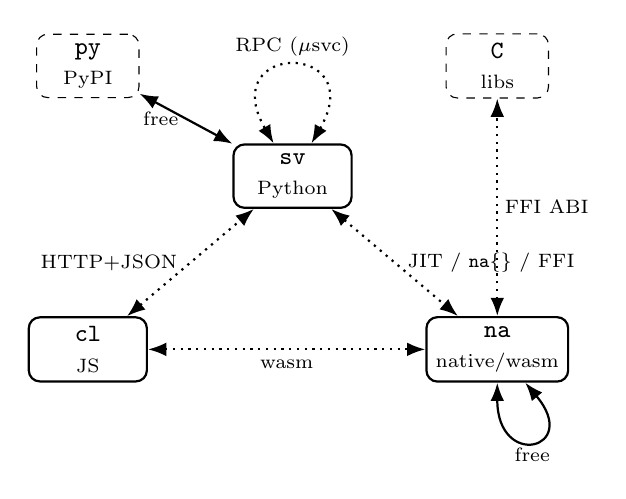
\begin{tikzpicture}[
  font=\small,
  space/.style={draw, rounded corners, minimum width=15mm, minimum height=8mm,
                align=center, thick},
  ambient/.style={draw, dashed, rounded corners, minimum width=13mm,
                  minimum height=7mm, align=center},
  free/.style={-{Latex}, thick},
  marsh/.style={-{Latex}, thick, dotted},
]
\node[space] (sv) at (0,0) {\code{sv}\\\scriptsize Python};
\node[space] (cl) at (-2.6,-2.2) {\code{cl}\\\scriptsize JS};
\node[space] (na) at (2.6,-2.2) {\code{na}\\\scriptsize native/wasm};
\node[ambient] (py) at (-2.6,1.4) {\code{py}\\\scriptsize PyPI};
\node[ambient] (c)  at (2.6,1.4)  {\code{C}\\\scriptsize libs};

% free edges (solid)
\draw[free, {Latex}-{Latex}] (sv) -- (py) node[midway,left=-1pt] {\scriptsize free};
\draw[free, {Latex}-{Latex}] (na) to[out=-50,in=-90,looseness=8]
  node[below=-1pt] {\scriptsize free} (na);

% marshalled edges (dotted)
\draw[marsh, {Latex}-{Latex}] (sv) -- (na)
  node[midway,right=1pt] {\scriptsize JIT / \code{na\{\}} / FFI};
\draw[marsh, {Latex}-{Latex}] (cl) -- (sv)
  node[midway,left=1pt] {\scriptsize HTTP+JSON};
\draw[marsh, {Latex}-{Latex}] (cl) -- (na)
  node[midway,below] {\scriptsize wasm};
\draw[marsh, {Latex}-{Latex}] (na) -- (c)
  node[midway,right=-1pt] {\scriptsize FFI ABI};
\draw[marsh, {Latex}-{Latex}] (sv) to[out=60,in=120,looseness=8]
  node[above] {\scriptsize RPC ($\mu$svc)} (sv);
\end{tikzpicture}
\caption{Jac's codespaces and ambient ecosystems. Solid arrows are
\emph{free} in-codespace calls (nothing serialized); dotted arrows are the
\emph{marshalled} boundaries JacInteropBench characterizes---each becomes an
RPC, an FFI thunk, or a WebAssembly import/export.}
\label{fig:overview}
\end{figure}

\begin{table}[t]
\caption{Boundary $\rightarrow$ kernel map. Prefix \code{iop\_*} = in-process
native bridge (family~1), \code{xop\_*} = cross-runtime (family~2),
\code{base\_*} = a named free floor. The ``real-world stand-in'' column names
each kernel's design target and analogue; as implemented the enabled cells are
synthetic microprograms, so that column is \emph{aspirational}---though the
callee-work sweep (Section~\ref{sec:sweep}) and the \code{xop\_feed\_payload}
payload sweep (Section~\ref{sec:payload}) now realize the two scaling axes.}
\label{tab:map}
\centering
\small
\begin{tabular}{@{}llll@{}}
\toprule
Boundary & Wire & Kernel(s) & Real-world stand-in \\
\midrule
\code{sv}$\rightarrow$\code{sv} & free & \code{base\_call} & Python-call floor \\
\code{sv}$\leftrightarrow$\code{py} & free & \code{base\_pyimport} & NumPy/sklearn floor \\
\code{sv}$\rightarrow$\code{na} & JIT & \code{iop\_call} & Python calls native \\
\code{na}$\rightarrow$\code{sv} & \code{na\{\}} & \code{iop\_cb} & native calls back \\
\code{sv}$\leftrightarrow$\code{na} & JIT & \code{iop\_symmetric} & placement dial \\
\code{na}$\leftrightarrow$\code{C} & FFI ABI & \code{iop\_ffi\_scalar} & libm \\
& & \code{iop\_ffi\_struct} & raylib, SQLite \\
& & \code{iop\_ffi\_vtable} & CEF callbacks \\
\code{sv}$\rightarrow$\code{sv} & HTTP+JSON & \code{xop\_svc\_split} & billing fan-out \\
& HTTP+JSON \code{[N]} & \code{xop\_feed\_payload} & typed feed payload \\
\code{cl}$\leftrightarrow$\code{sv} & HTTP+JSON & \code{xop\_feed} & littleX feed \\
\code{cl}$\rightarrow$\code{na} & wasm export & \code{xop\_wasm\_call} & PolyBench in browser \\
\bottomrule
\end{tabular}
\end{table}

Table~\ref{tab:map} lists the surface. The split into two harness families is not
cosmetic: it follows from what a boundary requires of the measurement harness. A
native bridge lives \emph{inside} one process---an in-process JIT or an
ahead-of-time native binary---so a command adapter can drive it directly. A
cross-runtime boundary requires a \emph{second} runtime---a live Jac server, a
generated JavaScript client, a Node WebAssembly host---so a host adapter must own
that runtime's lifecycle: allocate a port, start it, poll readiness, capture
logs, reset state between variants, and terminate-then-kill in every exit path.
The two families share one parsing, aggregation, and oracle module
(\code{common.jac}) but keep their build and host lifecycles separate.

Table~\ref{tab:profiles} is the conceptual spine of the characterization: it
names, per boundary, the \emph{dominant cost} a workload pays and the compiler
strategy that cost licenses. It is a taxonomy, not a measured policy---we do not
yet implement automatic strategy selection---but it states what a synechic
compiler is positioned to decide once each cost is measured, and it organizes
which cost each kernel in Table~\ref{tab:map} is designed to expose.

\begin{table}[t]
\caption{Boundary cost profiles. The dominant cost defines the workload class;
the enabled strategy is what owning both sides of the crossing lets a compiler
choose. Strategy selection is design-implication (Section~\ref{sec:implications}),
not a measured result.}
\label{tab:profiles}
\centering
\small
\begin{tabular}{@{}lll@{}}
\toprule
Boundary & Dominant cost & Enabled strategy \\
\midrule
\code{cl}$\rightarrow$\code{sv} & network + JSON ser. & batch / migrate / cache \\
\code{sv}$\leftrightarrow$\code{na} & FFI transition + marshal & inline vs.\ copied thunk \\
\code{na}$\rightarrow$\code{sv} & callback + runtime entry & hoist / amortize round trip \\
\code{sv}$\rightarrow$\code{sv} & RPC + placement & co-locate vs.\ split \\
\code{na}$\leftrightarrow$\code{C} & ABI class (register/\code{byval}) & pass-by-value vs.\ pointer \\
\code{cl}$\rightarrow$\code{na} & wasm import + BigInt copy & keep compute in-runtime \\
\bottomrule
\end{tabular}
\end{table}

\section{Methodology}
\label{sec:method}

\subsection{The kernel contract}

Every kernel obeys a load-bearing output contract inherited from \code{ownbench}
and extended for boundary crossings. Each invocation prints exactly one non-empty
\emph{canonical digest} line, exactly one effective \code{ns=$\langle$integer$\rangle$}
timing line, and zero or more unique integer \code{m:$\langle$key$\rangle$=$\langle$value$\rangle$}
metric lines. The parser strips both \code{ns=} and \code{m:} lines before
comparing digests, and rejects missing or multiple timing lines, duplicate
metrics, a changing metric-key set, or a nondeterministic digest.

Determinism is enforced by construction: fixed linear-congruential-generator
(LCG) seeds, sorted iteration, fresh or reset state per variant, and no clocks,
generated identifiers, transport envelopes, or object addresses in the digest.
Each run selects exactly one named work size, so a single run reports per-call or
per-batch time \emph{at that size only}. Invocations within a run are interleaved
per variant (paired sampling) so that machine drift hits both sides of a
comparison evenly.

\subsection{The differential-identity oracle}

The suite's central discipline is that \emph{identity is never checked against a
generic floor}. Every marshalled cell names an exact reference twin that runs the
same operation over the same deterministic input without the crossing. The
\code{free} variant of \code{iop\_call} runs an LCG checksum in ordinary
\code{sv}; the \code{bridge} variant runs the identical checksum inside a
\code{na\{\}} block. Both must emit the byte-identical canonical digest
\code{call:263997602}. When they do, three facts are witnessed simultaneously:
the marshalling preserved semantics, the native code path is functionally
equivalent to the server path, and no compiler change silently perturbed either.
This is the load-bearing contribution. A speedup is interesting; a
byte-identical digest across a marshalled seam, checked on every commit, is a
guarantee.

The oracle's reach is best seen in one number. The same deterministic LCG
checksum, \code{263997602}, is reproduced byte-for-byte across six kernels
spanning every wire in the suite---\code{sv} and \code{na} execution
(\code{iop\_call}, \code{iop\_symmetric}), a native$\rightarrow$server callback
(\code{iop\_cb}), two HTTP+JSON RPC paths (\code{xop\_feed},
\code{xop\_svc\_split}), and a \code{wasm32} export (\code{xop\_wasm\_call}).
One workload, six runtimes and transports, one canonical value: that identity is
the correctness claim the whole suite is built to defend.

Concretely, the continuous-integration gate (\code{ci\_bridges.sh}) runs the
enabled kernels at small sizes, filters out both \code{ns=} and \code{m:} lines,
and asserts canonical-digest identity across each declared twin group plus a set
of named structural invariants (Section~\ref{sec:audit}). \emph{Timing values
never gate CI.} A regression is a semantic divergence or a broken structural
invariant, never a slow number on a noisy runner. The same scalar pair also
lives as a standalone compiler regression test
(\code{test\_interopbench\_bridges.jac}) that invokes both paths through
\code{python -m jaclang run} and asserts digest identity, with no GNU-time,
NumPy, C-compiler, Node, server, or WebAssembly prerequisite.

\subsection{Structural audits}
\label{sec:audit}

Beyond digest identity, the suite records named \emph{structural} facts about the
generated code (\code{interop\_audit.json}). Manifest/wrapper audits are enabled
for the two mixed-JIT scalar cells (\code{iop\_call}, \code{iop\_cb}); the FFI
cells' IR/ABI assertions live in the compiler's existing owner tests
(\code{test\_abi\_lib}, \code{test\_native\_gen\_pass}) rather than in this
suite. For \code{iop\_call}, the audit
asserts the \code{InteropManifest} exports exactly \code{native\_checksum} and no
imports, that the generated Python wrapper contains exactly one
\code{get\_function\_address('native\_checksum')} lookup and one matching
\code{ctypes.CFUNCTYPE} signature, and that the pure-\code{sv} baseline
(\code{sv\_checksum}) generates \emph{no} native binding. For \code{iop\_cb}, it
additionally asserts one native import (\code{sv\_callback\_checksum}) and its
\code{\_\_jac\_interop\_py\_funcs\_\_} registration. These are compiler-drift
sentinels: they fail loudly if a codegen change adds a stray ctypes stub or
drops a trampoline, catching regressions that a purely behavioral oracle would
miss. Table~\ref{tab:audit} shows the concrete asserted facts; all matched on the
measured build.

\begin{table}[t]
\caption{Structural-audit facts (\code{interop\_audit.json}), expected =
actual on the measured build. Enabled for the two mixed-JIT scalar cells.}
\label{tab:audit}
\centering
\footnotesize
\setlength{\tabcolsep}{4pt}
\begin{tabular}{@{}lll@{}}
\toprule
Cell & Asserted fact & Count \\
\midrule
\code{iop\_call} & \code{native\_exports}=\{\code{native\_checksum}\} & 1 \\
                 & \code{get\_function\_address} lookup & 1 \\
                 & \code{ctypes.CFUNCTYPE} signature & 1 \\
                 & baseline \code{sv\_checksum} native bindings & 0 \\
\midrule
\code{iop\_cb}   & \code{native\_imports}=\{\code{sv\_callback\_checksum}\} & 1 \\
                 & \code{\_\_jac\_interop\_py\_funcs\_\_} reg. & 1 \\
                 & baseline \code{sv\_direct\_checksum} bindings & 0 \\
\bottomrule
\end{tabular}
\end{table}

\subsection{Oracle efficacy: a seeded-fault study}
\label{sec:oracleeval}

A correctness oracle is only a contribution if it catches faults, so we tested it
directly. We injected a corpus of $21$ seeded mutations into the crossing side of
seven twin groups (\code{iop\_call}, \code{iop\_cb}, \code{iop\_symmetric},
\code{iop\_ffi\_struct}, \code{iop\_ffi\_vtable}, \code{xop\_feed\_payload},
\code{xop\_svc\_split}), each modeling a target bug class: one-sided LCG/codegen
drift, argument-order and truncation errors at the boundary, dropped and
duplicated payload elements in RPC deserialization, C-ABI field truncation,
integer narrowing, byte-order swap, callback-trampoline argument swap, foreign
struct-declaration skew, boundary erasure (the reference side silently promoted to
native), a common-mode provider bug, and three result-preserving \emph{timing-only}
controls. Each mutation was applied in isolation, the cell's oracle group re-run at
the CI operating point, and digests compared exactly as the gate does; the
structural audit was run where applicable; the tree was reverted between mutations.

The oracle caught \textbf{all $14/14$ mutations that corrupted the crossing's
observable result} at CI sizes (Table~\ref{tab:oracleeval}), with \textbf{zero
false alarms} on the three timing-only mutations---confirming it is orthogonal to
timing, which is precisely why frequency pinning (Section~\ref{sec:controls}) is a
separate and necessary discipline. In one case it flagged a native-export
type-confusion fault (\code{return "oops"} from an \code{int}-typed export) that
the type checker itself accepted. Three faults escaped, and each marks a real
limit rather than a mechanism flaw: a \emph{common-mode} bug in provider source
shared by both twins is structurally invisible to any differential oracle; an
integer-narrowing bug in the C fixture is masked at CI and default input sizes
(its truncated sum only exceeds $16$ bits at $N\ge10{,}922$), so catch power is
input-domain-dependent; and an ABI declaration skew on a \emph{pass-through}
struct changed no observed byte and evaded both the oracle and the structural
audit---a latent hazard we report rather than hide. The structural audit earns its
keep on the complementary failure the oracle cannot see: erasing the
\code{sv}/\code{na} boundary leaves digests byte-identical while silently deleting
the phenomenon under measurement (per-call cost fell $41.2$ to $4.7$\,\textmu s),
and only the export-manifest gate detects it. Across all $17$ non-timing seeded
faults the oracle-plus-audit layer caught $15$; the oracle alone caught
$14/14$ of those that were observable at the measured sizes.

\begin{table}[t]
\caption{Seeded-fault evaluation of the differential-identity oracle. $21$
mutations on the crossing side of seven twin groups; CAUGHT = digests diverged,
TN = correctly passed (timing-only). The three escapes each delineate a scope
limit (common-mode, input-domain-masked, latent pass-through ABI skew).}
\label{tab:oracleeval}
\centering
\small
\begin{tabular}{@{}lrr@{}}
\toprule
Fault class & injected & caught \\
\midrule
Result-corrupting, observable at CI size & 14 & \textbf{14} \\
\quad(codegen/LCG drift, arg-order, truncation, & & \\
\quad dropped/dup element, field truncation, & & \\
\quad byte-swap, callback-arg swap, type confusion) & & \\
Timing-only (should \emph{not} fire) & 3 & 0 (correct) \\
Common-mode provider bug & 1 & 0 (undecidable) \\
Input-domain-masked narrowing & 1 & 0 at CI ($N{<}10{,}922$) \\
Pass-through ABI declaration skew & 1 & 0 (oracle \& audit blind) \\
Boundary erasure & 1 & audit-only \\
\bottomrule
\end{tabular}
\end{table}

\subsection{Provenance and spread}

Results are schema version~2. Every document carries a \code{provenance} block
(host, platform, machine, CPU count, Python version, UTC capture time) so a
number is never quoted without the machine it came from. Each cell records
\code{samples}, \code{median\_ns}, \code{min\_ns}, \code{max\_ns},
\code{stdev\_ns}, and \code{iqr\_ns}. What is deliberately \emph{not} computed:
confidence intervals, ratio uncertainty, or an outlier policy---spread is
reported, not gated. Results also label \code{command\_adapter},
\code{timing\_source}, and \code{rss\_scope}; cross-runtime cells that cannot
share a clock label \code{timing\_source} \emph{per variant} rather than stamping
one label over a mixed pair.

\subsection{Measurement controls}
\label{sec:controls}

Family-1 timings and the two loopback RPC cells of family~2 are captured with the
CPU frequency \emph{pinned}: the governor is fixed to \code{performance} on all
cores and Intel Turbo Boost is disabled (\code{intel\_pstate/no\_turbo=1}). This
is load-bearing. An earlier uncontrolled capture (default \code{powersave}
governor, turbo on) produced two artifacts we now attribute entirely to
frequency non-determinism, not to the toolchain---a concrete instance of
measurement context producing wrong data without anything obviously
wrong~\cite{mytkowicz}. First, the same \code{sv}-resident
loop fit to two different slopes on different runs ($\approx$$88$ vs.\
$\approx$$185$\,ns/iter)---base clock vs.\ boost clock on the same code. Second,
because a boosted clock \emph{droops} thermally over an eight-minute sweep (early
points fast, late points slow), the linear fits tilted and extrapolated to
negative intercepts, inflating the callback twin-gap to $\approx$$5.4$\,\textmu s.
Under the pinned clock every \code{sv}-resident slope converges to
$212$--$217$\,ns/iter, all intercepts are positive, and the callback gap settles
at $\approx$$2.0$\,\textmu s.

The consequence for how results should be read: \emph{ratios} (placement
$42\times$, the cross-runtime floors) are reproducible and portable, whereas the
\emph{absolute} nanosecond figures are specific to this CPU
(Intel Core Ultra~7~255H) at its pinned base clock---disabling turbo halves the
clock, so the \code{direct} baseline moves from $\approx$$385$ to
$\approx$$805$\,\textmu s, a clean $2.09\times$. We therefore quote absolutes only
as ``this microprogram, at this size, on this machine,'' and rest every
comparative claim on a ratio. Run-to-run stability is characterized rather than
assumed: three repeats of the RPC cells give a ratio coefficient of variation of
$3.0$--$3.7\%$, with the \code{direct} baseline stable to $0.3\%$, locating all
residual jitter in the RPC numerator (loopback and V8 scheduling), which no
governor setting removes. Full provenance, the pinned-governor dataset, and the
superseded uncontrolled captures are released together.

\section{Kernels}
\label{sec:kernels}

\paragraph{Family~1: native bridges (\code{iop\_*})}
\code{iop\_call} is the vertical slice: one mixed source runs a deterministic
scalar LCG checksum in \code{sv} (\code{free}) and in \code{na\{\}}
(\code{bridge}). It is an \emph{execution-placement} benchmark---the ratio blends
the \code{sv$\rightarrow$na} crossing with native-vs-server execution speed, not
isolated boundary cost. \code{iop\_cb} isolates the crossing: both variants run
the work in \code{sv}, and only the \code{bridge} path adds a
native$\rightarrow$server callback round trip, making it the cleanest boundary
cell. \code{iop\_symmetric} sweeps all four placements (\code{sv\_local},
\code{sv\_to\_na}, \code{na\_local}, \code{na\_to\_sv}) over identical callee
work. The three \code{iop\_ffi\_*} kernels exercise the \code{na$\leftrightarrow$C}
ABI through a deterministic \code{C} fixture: \code{iop\_ffi\_scalar} churns
\code{libm} \code{sqrt}; \code{iop\_ffi\_struct} passes
\code{\_Static\_assert}ed 4/12/16/24/44-byte structs by value across System~V
INTEGER and MEMORY classes; \code{iop\_ffi\_vtable} has \code{C} invoke a Jac
callback through a \code{\_\_clibcb} trampoline.

\paragraph{Family~2: cross-runtime (\code{xop\_*})}
\code{xop\_svc\_split} places an \code{sv import from billing} between two
loopback \code{jac start} deployments, with direct in-process dispatch as its
twin. \code{xop\_feed\_payload} uses the same loopback \code{sv$\rightarrow$sv}
seam but varies the returned \code{list[$N$]} cardinality rather than callee work,
isolating a per-element serialization slope (Section~\ref{sec:payload}).
\code{xop\_feed} drives a scalar provider through a generated JavaScript
client over HTTP+JSON. \code{xop\_wasm\_call} compiles an integer kernel to
\code{wasm32} and invokes it from a Node host, against a native bridge as
reference. As Section~\ref{sec:threats} details, the scalar cross-runtime cells
are honest \emph{floors}, not microservice or same-source native-vs-wasm
measurements; \code{xop\_feed\_payload} adds the one payload-scaling curve.

\section{Results}
\label{sec:results}

All numbers below were captured on host \code{zaitop}: Linux~6.18 x86\_64,
16~cores, CPython~3.14.6. Single-size tables use the small work size
(\code{args = 200, 20}); Section~\ref{sec:sweep} sweeps eight callee-work sizes
and Section~\ref{sec:payload} sixteen payload cardinalities. All family-1 cells
(the single-size bridge table below, the \code{iop\_ffi\_*} cells, and the
eight-point sweep of Section~\ref{sec:sweep}), the three family-2 cross-runtime
cells, and the payload sweep (Section~\ref{sec:payload}) are captured under
the pinned governor with turbo disabled (Section~\ref{sec:controls}), as medians
of three runs at $n{=}20$. Every cell's variants produced byte-identical
canonical digests---the oracle passed for all ten measured kernels at every size,
independent of clock.

\subsection{Native bridges}

Table~\ref{tab:bridges} reports the family-1 results (median of three
pinned-governor runs at $n{=}20$, Section~\ref{sec:controls}), anchored by the
named free floor \code{base\_call}: a bare \code{sv$\rightarrow$sv} call over the
same LCG leaf measures $40{,}144$\,ns/call at this size and emits the same
\code{call:263997602} digest as the rest of the suite. So \code{iop\_call}'s
$41{,}531$\,ns \code{free} reference is essentially the bare \code{sv}-call floor
plus noise---the \code{sv$\rightarrow$na} comparisons below are against a real
floor, not inflated server code. (The companion \code{sv$\leftrightarrow$py}
floor \code{base\_pyimport}---a \code{sv}$\rightarrow$Python call into an imported
NumPy \code{arange}+\code{sum} leaf, NumPy~2.5.1 provisioned into the \code{jac}
runtime---measures $3{,}413$\,ns/call at the same $200/20$ size, median of $15$
under the pinned clock, digest \code{pyimport:398210}. It is not comparable to
\code{base\_call} as a multiple, since NumPy's vectorized C leaf and the
interpreted-\code{sv} LCG leaf do different work; it stands as the imported-C-extension
boundary floor in its own right.) Four findings stand out.

\emph{Native execution is fast, but that is placement, not boundary cost.}
\code{iop\_call} runs the LCG $8.7\times$ faster inside \code{na\{\}}
($4{,}747$\,ns/call) than in \code{sv} ($41{,}531$\,ns/call), and
\code{iop\_symmetric}'s \code{na\_local} floor ($1{,}279$\,ns/call) is $32\times$
below its \code{sv\_local} twin. These ratios are dominated by how fast each
runtime executes the kernel, not by what the crossing costs.

\emph{The crossing itself is cheap.} \code{iop\_cb}, which holds execution in
\code{sv} and adds only a native$\rightarrow$server callback round trip, costs
$45{,}712$\,ns/call against a $40{,}533$\,ns/call reference---a $1.13\times$
ratio, i.e.\ the round trip adds roughly $13\%$. The median ratio is stable
across the three pinned runs ($1.12$/$1.15$/$1.12\times$, CV $1.2\%$) and the two
medians are cleanly separated, though at $n{=}20$ the distribution tails do touch
(pooled reference \code{max} $896{,}323$ vs.\ bridge \code{min} $872{,}995$\,ns),
so we read this as a $\approx$$13\%$ effect, not a hairline one. The $\approx$$5$\,\textmu s
absolute gap this single size implies exceeds the fixed $\approx$$2.0$\,\textmu s
twin-gap intercept that the work sweep fits (Section~\ref{sec:sweep}); the excess
is low-work curvature, which is exactly why the fitted intercept---not the raw
single-size ratio---is the load-bearing measure of the crossing cost. This is the
suite's cleanest single-size statement of boundary overhead, resolved into that
fixed intercept next.

\emph{The C ABI is close to free for scalars and callbacks---but not zero.} The
integer per-call metric (\code{m:per\_ffi\_call\_ns}) floors both FFI scalar and
trampoline costs to $2$--$3$\,ns, which understates a real sub-nanosecond
premium visible in the batch medians: \code{iop\_ffi\_vtable}'s
\code{C$\rightarrow$Jac} trampoline adds $11.7\%$ to batch wall time
($13{,}277$ vs.\ $11{,}885$\,ns over the same call count), and
\code{iop\_ffi\_scalar}'s \code{sqrt} adds $21.8\%$ over its arithmetic reference
($14{,}131$ vs.\ $11{,}605$). The trampoline is cheap, not free; we read it off
the batch wall time, not the quantized per-call integer. Struct-by-value is
where marshalling shows plainly: \code{iop\_ffi\_struct} makes ten \code{C} calls
per outer call across five heterogeneous shapes, averaging $17$\,ns per foreign
call---an average across INTEGER- and MEMORY-class shapes, not a per-shape cost,
and the reason its batch median ($713{,}462$\,ns) sits $6.9\times$ above the
computed reference.

\emph{Run-to-run variance is placement-dependent, not crossing-dependent.} The
sharpest workload observation in the family-1 data is in the dispersion, not the
medians. Every \code{sv}-resident variant is noisy---\code{iop\_call} free
\code{stdev} $36{,}858$\,ns, \code{na\_to\_sv} $26{,}096$, \code{iop\_cb} bridge
$33{,}311$---while every \code{na}-resident variant is roughly an order of
magnitude quieter: \code{iop\_call} bridge \code{stdev} $7{,}275$,
\code{na\_local} $1{,}403$, and the \code{iop\_ffi\_*} reference cells
$31$--$3{,}142$\,ns. Run-to-run jitter tracks \emph{where the work executes}:
CPython scheduling, not the marshalled seam, dominates variance. This is why
paired, interleaved sampling matters---it puts that CPython jitter on both sides
of every comparison evenly. We report \code{min}/\code{max}/\code{stdev}/\code{iqr}
per cell and gate on none of them (Section~\ref{sec:method}); the native-path
ratios above are $8$--$32\times$, read off medians whose few-percent spread is far
too small to swallow them.

\begin{table}[t]
\caption{Family~1 native bridges. Median wall time and the kernel's own
per-call metric (\code{ns}). Digests identical within every cell.}
\label{tab:bridges}
\centering
\small
\setlength{\tabcolsep}{4.5pt}
\begin{tabular}{@{}llrr@{}}
\toprule
Cell & Variant & Median (ns) & per-call (ns) \\
\midrule
\code{iop\_call} & free (\code{sv} ref) & 830{,}632 & 41{,}531 \\
                 & bridge (\code{na})   & 94{,}961  & 4{,}747 \\
\midrule
\code{iop\_cb}   & free (\code{sv} ref)        & 810{,}681 & 40{,}533 \\
                 & bridge (\code{sv}$\to$\code{na}$\to$\code{sv}) & 914{,}256 & 45{,}712 \\
\midrule
\code{iop\_symmetric} & sv\_local & 815{,}519 & 40{,}775 \\
                      & sv\_to\_na & 97{,}456 & 4{,}872 \\
                      & na\_local  & 25{,}592 & 1{,}279 \\
                      & na\_to\_sv & 814{,}722 & 40{,}735 \\
\midrule
\code{iop\_ffi\_scalar} & ref (int math)   & 11{,}605 & 2 \\
                        & ffi (\code{sqrt}) & 14{,}131 & 3 \\
\midrule
\code{iop\_ffi\_struct} & ref (computed)   & 104{,}128 & 2 \\
                        & ffi (struct ABI) & 713{,}462 & 17 \\
\midrule
\code{iop\_ffi\_vtable} & ref (direct Jac)      & 11{,}885 & 2 \\
                        & ffi (\code{C}$\to$Jac) & 13{,}277 & 3 \\
\bottomrule
\end{tabular}
\end{table}

\subsection{Cross-tool FFI baseline}
\label{sec:xtool}

A per-foreign-call cost is only interpretable against a comparand. The
\code{iop\_ffi\_scalar} kernel calls \code{libm}'s \code{sqrt} from Jac's native
codespace; Jac's mixed-JIT path emits a \code{ctypes.CFUNCTYPE} thunk
(Section~\ref{sec:audit}), so the natural controlled A/B is the \emph{same} libm
\code{sqrt}, over the \emph{same} deterministic loop, called from Python's
standard FFI mechanisms---\code{ctypes} and \code{cffi}---and, to answer the
sharper objection that these conflate mechanism with interpreter cost, from a
matched \code{pybind11} module, a \code{PyO3} (Rust) module, and a hand-written
\code{METH\_O} C extension, plus each side's no-FFI arithmetic floor.

Table~\ref{tab:xtool} reports two measurements per toolchain. The \emph{matched}
column is per-foreign-call cost under the kernel's exact loop
(\code{int(sqrt(float(i*i)))}, warmed, digest-verified); the \emph{isolated}
column strips the loop by differencing a tight call loop against an empty one,
leaving the boundary alone. The gap between them is the whole story. In the
matched column Jac-native FFI ($3.1$\,ns) is $\approx$$50\times$ cheaper than a
pybind11 wrapper ($163$\,ns) or a raw \code{METH\_O} C extension ($136$\,ns) and
$\approx$$150\times$ cheaper than \code{ctypes} ($475$\,ns)---but those matched
figures are dominated by \emph{CPython interpreter dispatch, not the binding
mechanism}: a \emph{noop} C function costs the same as \code{sqrt} in both
pybind11 and the C extension ($\Delta<0.5$\,ns), and a pure-Python identity
lambda in the same loop costs $139$\,ns. Isolating the call itself tells the
honest story: the Python$\rightarrow$C boundary is $\approx$$25$\,ns for a raw
\code{METH\_O} C extension, $\approx$$40$\,ns for PyO3, and $\approx$$54$\,ns for
pybind11---a narrow $25$--$54$\,ns band across hand-written and generated binding
layers---against $\approx$$3$\,ns per whole iteration (loop, call, and arithmetic
together) for Jac-native FFI, and an order of magnitude above them all,
\code{ctypes} at $\approx$$367$\,ns. So Jac's advantage over the best CPython-native
bindings on \emph{mechanism} cost is roughly an order of magnitude, not the
$100\times$-class ratio \code{ctypes} exhibits. Part of even the $25$\,ns
raw-extension floor is \code{PyFloat} boxing and refcounting that any CPython
extension must pay---runtime tax, not binding-generator overhead. Every variant
reconstructs the byte-identical digest \code{sqrt:402000}, so the
differential-identity oracle now spans \emph{toolchains}: PyO3, pybind11, the C
extension, \code{ctypes}, \code{cffi}, and Jac-native are provably computing one
value from the same foreign calls.

\begin{table}[t]
\caption{Cross-tool FFI: same \code{libm} \code{sqrt}, same loop, same digest
\code{sqrt:402000}. \emph{matched} = per foreign call under the kernel's loop
($n{=}200$, median of five); \emph{isolated} = per-call boundary only (tight call
loop minus empty loop). The matched$\to$isolated drop exposes how much is
CPython dispatch rather than binding mechanism.}
\label{tab:xtool}
\centering
\small
\begin{tabular}{@{}llrr@{}}
\toprule
Toolchain & Path & matched & isolated \\
\midrule
Jac \code{na}        & FFI (\code{sqrt})  & $3.1$ & --- \\
Jac \code{na}        & ref (no FFI)       & $2.5$ & --- \\
raw C-ext (\code{METH\_O}) & FFI (\code{sqrt}) & $136$ & $25$ \\
PyO3 (Rust)          & FFI (\code{sqrt})  & $145$ & $40$ \\
pybind11             & FFI (\code{sqrt})  & $163$ & $54$ \\
Python \code{cffi}   & FFI (\code{sqrt})  & $314$ & --- \\
Python \code{ctypes} & FFI (\code{sqrt})  & $475$ & $367$ \\
Python               & ref (no FFI)       & $39$  & $\approx$$22$ \\
\bottomrule
\end{tabular}
\end{table}

\subsection{Cross-runtime}

Table~\ref{tab:xruntime} reports the family-2 results, all three cells
captured under the pinned clock (Section~\ref{sec:controls}) as medians of three
runs at $n{=}20$ interleaved invocations. For the two loopback RPC cells (\code{xop\_svc\_split},
\code{xop\_feed}) the run-to-run ratio CV is $\le$$4\%$ (the \code{direct}
baseline is stable to $0.3\%$, so what jitter remains lives entirely in the RPC
numerator); the \code{wasm32} cell is tighter still (crossing median CV
$<$$4\%$, native CV $<$$0.1\%$). The marshalled crossings are one to two-plus
orders of magnitude more expensive than the direct dispatch they replace: a
loopback HTTP+JSON RPC (\code{xop\_svc\_split}) costs $374\times$ its in-process
twin and a generated-client feed (\code{xop\_feed}) $241\times$ its direct
provider call, while a \code{wasm32} export (\code{xop\_wasm\_call}) is
$6.8\times$ a native bridge under an asymmetric host loop.

These RPC ratios are floors \emph{for the shipped deployment path}, and we are
explicit about why. We decomposed the per-call RPC floor---$\approx$$13$\,ms
measured directly on the client path against a warm provider, which the
payload-sweep fit (Section~\ref{sec:payload}) extrapolates to a $\approx$$15$\,ms
intercept, the $\approx$$2$\,ms difference being per-invocation warm-up folded
into the fit---by timing the same provider four ways (Table~\ref{tab:rpcfloor}):
the \code{sv~import} client path ($\approx$$13$\,ms), raw HTTP to the same server
with a new connection per call ($\approx$$6$\,ms), raw HTTP over a persistent
connection ($\approx$$6$\,ms), and---as a light-endpoint control---raw HTTP to a
bare one-route \code{http.server} computing the identical result
($\approx$$1.1$\,ms). Keep-alive versus per-call connect makes no measurable
difference, so loopback TCP setup is \emph{not} the cost. Two terms remain.
First, $\approx$$5$\,ms of \emph{application-framework dispatch}: the provider is
a full \code{jac start} server whose route table spans \code{/admin/*},
\code{/sso/*}, telemetry and \code{/user/*}, so every \code{feed\_batch} call
pays routing, auth-middleware and request-context overhead the bare endpoint does
not---measured directly as the $\approx$$6$\,ms server path minus the
$\approx$$1.1$\,ms minimal endpoint. Second, $\approx$$7$\,ms of client-path
overhead in \code{sv~import} (obtained by subtraction, $13-6$; connection,
validation and JSON marshalling). Both are real costs a Jac user on today's
shipped path pays, but neither is intrinsic to a loopback RPC in general---a
minimal endpoint and a tuned client, as the $\approx$$1.1$\,ms control shows, are
far cheaper---so the $374\times$/$241\times$ figures measure Jac's current hosted
path, not the price of an RPC boundary as such. What the sweep \emph{does} isolate
cleanly is the per-element serialization slope (Section~\ref{sec:payload}), which
is unaffected by this fixed framework floor.

The RPC crossing-side spread is also wide (the RPC medians vary $189$--$309$\,M\,ns
run to run), so we read those as \emph{floors}, not precise ratios---and they
remain the least apples-to-apples comparisons in the suite, since the two sides
do not share a clock (each carries its own \code{timing\_source}). Every
cross-runtime cell's digests were byte-identical across all samples.

\begin{table}[t]
\caption{Family~2 cross-runtime. Direct twin vs.\ marshalled crossing, all cells
medians of three pinned-governor runs at $n{=}20$ (Section~\ref{sec:controls}).
Timing sources differ per variant (see text); the RPC crossing-side spread is
wide, so those ratios are floors.}
\label{tab:xruntime}
\centering
\small
\begin{tabular}{@{}lrrr@{}}
\toprule
Cell & Direct med.\ (ns) & Crossing med.\ (ns) & Ratio \\
\midrule
\code{xop\_svc\_split} & 805{,}553 & 300{,}949{,}052 & $374\times$ \\
\code{xop\_feed}      & 805{,}204 & 193{,}703{,}449 & $241\times$ \\
\code{xop\_wasm\_call} & 19{,}429  & 132{,}647       & $6.8\times$ \\
\bottomrule
\end{tabular}
\end{table}

\begin{table}[t]
\caption{Decomposing the per-call RPC floor ($\approx$$13$\,ms on the client
path; the payload-sweep fit intercept is $\approx$$15$\,ms including per-invocation
warm-up). Same result computed four ways, small $N$, pinned clock. Keep-alive
vs.\ new-connection is within noise (TCP setup is not the cost); the
minimal-endpoint control isolates $\approx$$5$\,ms of \code{jac start}
application-framework dispatch, and the client path adds $\approx$$7$\,ms of
\code{sv~import} overhead---neither intrinsic to a loopback RPC in general.}
\label{tab:rpcfloor}
\centering
\small
\begin{tabular}{@{}lrl@{}}
\toprule
Path & per-call & isolates \\
\midrule
\code{sv~import} client (measured)   & $\approx$$13$\,ms  & app-server + client overhead \\
raw HTTP, new connection/call        & $\approx$$6$\,ms   & app-server + TCP connect \\
raw HTTP, persistent connection      & $\approx$$6$\,ms   & app-server dispatch only \\
raw HTTP, minimal one-route endpoint & $\approx$$1.1$\,ms & HTTP + JSON + trivial routing \\
\bottomrule
\end{tabular}
\end{table}

\subsection{Separating fixed cost from callee work}
\label{sec:sweep}

A single work size cannot tell a fixed per-call crossing cost apart from
per-iteration execution cost. To separate them we sweep the callee work
parameter across eight sizes ($w\in\{25,\dots,3200\}$ LCG iterations/call at
$40$ calls, median of $20$ timed samples per point through the same \code{jac run}
adapter, under the pinned governor and disabled turbo of
Section~\ref{sec:controls}) and fit each variant's per-call time to
$t(w)\approx t_0 + s\cdot w$. The intercept $t_0$ is the per-call
boundary/dispatch cost independent of callee work; the slope $s$ is the
per-iteration execution cost. All fits are near-perfect lines
($R^2\ge0.999$ for every \code{sv}-resident series; Table~\ref{tab:fits}).

Two facts fall straight out. First, \emph{slope is bimodal by placement}:
\code{na}-resident execution runs at $\approx$$5$\,ns/iter
(\code{iop\_call} bridge, \code{na\_local}, \code{sv\_to\_na}) while
\code{sv}-resident execution runs at $\approx$$212$\,ns/iter---a
$\approx$$42\times$ gap ($211.95/5.04$) that is a property of \emph{where the
work runs}, not of the crossing. This ratio is the robust, reproducible headline;
its absolute ns values are clock-specific (Section~\ref{sec:controls}). Second,
\emph{the callback boundary is a fixed per-call cost, not a percentage}. In
\code{iop\_cb} the \code{free} and \code{bridge} slopes are statistically
identical ($211.95$ vs.\ $212.89$\,ns/iter, within $0.4\%$): the two variants do
the same work, so their fitted lines are parallel and separated by a fixed
intercept gap of $\approx$$2.0$\,\textmu s---the pure per-call callback cost.
That fixed cost is why the \code{iop\_cb} crossing
amortizes: once the callee does real work ($w\gtrsim800$) the per-call time is
dominated by the shared $\approx$$212$\,ns/iter slope and the bridge/reference
ratio settles to $\approx$$1.0$ (Figure~\ref{fig:decay}); at small $w$ the ratio
is dominated by timer noise rather than the boundary. The
$1.13\times$ single-size headline is not a property of the boundary; it is a
small fixed cost seen at one small size that vanishes once the callee does real
work. \code{iop\_symmetric}
makes the decomposition visible in one cell: \code{sv\_to\_na} runs at the
\emph{native} slope ($5.10$) yet carries a $\approx$$3.7$\,\textmu s crossing
intercept, so entering \code{na} pays a one-time per-call toll and then executes
$42\times$ faster per iteration---precisely the trade a placement decision must
weigh.

\begin{table}[t]
\caption{Linear fits $t(w)=t_0+s\cdot w$ of per-call time (ns) vs.\ callee work,
eight sizes, median of $20$ timed samples per point under a pinned CPU governor
and disabled turbo (Section~\ref{sec:controls}). $t_0$ is the per-call
boundary/dispatch intercept, $s$ the per-iteration execution slope. Absolute
$t_0$ is an extrapolation (the small $\approx$$-100$\,ns values are low-work
loop curvature, not negative cost); the load-bearing quantity is the intercept
\emph{gap} between twinned variants (see text). For \code{iop\_call} and
\code{iop\_cb}, \code{free} executes in \code{sv} and \code{bridge} in
\code{na}; the $\approx$$5$ vs.\ $\approx$$212$\,ns/it slopes read off the
executing codespace. The low $R^2$ ($.974$, \code{iop\_call} bridge) is the
native path measured near the timer noise floor: at $\approx$$7.9$\,ns/it the
slope is real but low-SNR, and it is corroborated by three independent
\code{na}-resident series ($7.92/5.10/5.04$), so no single fit is load-bearing.}
\label{tab:fits}
\centering
\footnotesize
\setlength{\tabcolsep}{4pt}
\begin{tabular}{@{}llrrr@{}}
\toprule
Cell & Variant & $t_0$ (ns) & $s$ (ns/it) & $R^2$ \\
\midrule
\code{iop\_call} & free    & $4987$ & $216.59$ & $.996$  \\
                 & bridge  & $4936$ & $7.92$   & $.974$  \\
\midrule
\code{iop\_cb}   & free    & $1910$ & $211.95$ & $1.000$ \\
                 & bridge  & $3918$ & $212.89$ & $1.000$ \\
\midrule
\code{iop\_symmetric} & sv\_local  & $-126$  & $211.81$ & $1.000$ \\
                      & sv\_to\_na & $3686$  & $5.10$   & $1.000$ \\
                      & na\_local  & $137$   & $5.04$   & $1.000$ \\
                      & na\_to\_sv & $-112$  & $213.90$ & $1.000$ \\
\bottomrule
\end{tabular}
\end{table}

\begin{figure}[t]
\centering
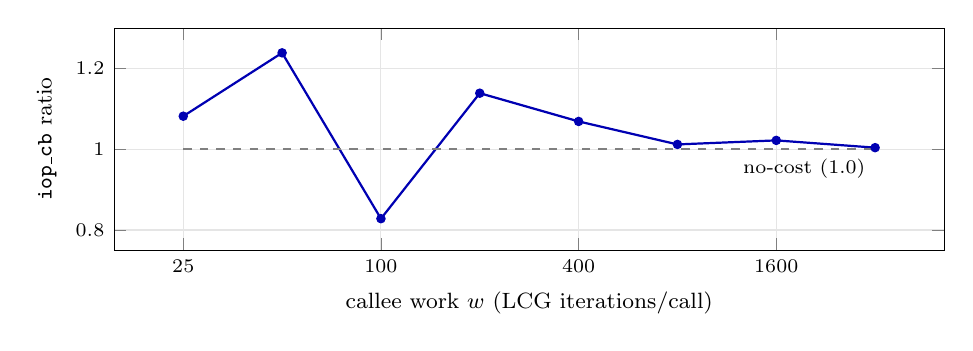
\begin{tikzpicture}
\begin{semilogxaxis}[
  width=\columnwidth, height=4.4cm,
  log basis x=2,
  xlabel={callee work $w$ (LCG iterations/call)},
  ylabel={\code{iop\_cb} ratio},
  xtick={25,100,400,1600}, xticklabels={25,100,400,1600},
  ymin=0.75, ymax=1.3,
  ytick={0.8,1.0,1.2},
  grid=both, grid style={gray!20},
  tick label style={font=\scriptsize}, label style={font=\footnotesize},
  every axis plot/.append style={thick},
]
\addplot[mark=*,mark size=1.3pt,blue!70!black] coordinates {
  (25,1.082)(50,1.239)(100,0.828)(200,1.139)(400,1.069)(800,1.012)(1600,1.022)(3200,1.004)
};
\addplot[dashed,gray] coordinates {(25,1.0)(3200,1.0)};
\node[anchor=north east,font=\scriptsize] at (axis cs:3200,1.0) {no-cost (1.0)};
\end{semilogxaxis}
\end{tikzpicture}
\caption{The \code{iop\_cb} bridge/reference ratio converges to $\approx$$1.0$
once callee work grows ($w\gtrsim800$), because the callback crossing is a
\emph{fixed} $\approx$$2.0$\,\textmu s per-call cost (Table~\ref{tab:fits}), not
a proportional overhead. Under pinned-clock timing the small-$w$ ratios are
noise-dominated (they scatter $0.83$--$1.24$); the fixed cost is established by
the twin-gap fit, not by these raw ratios.}
\label{fig:decay}
\end{figure}

\begin{figure}[t]
\centering
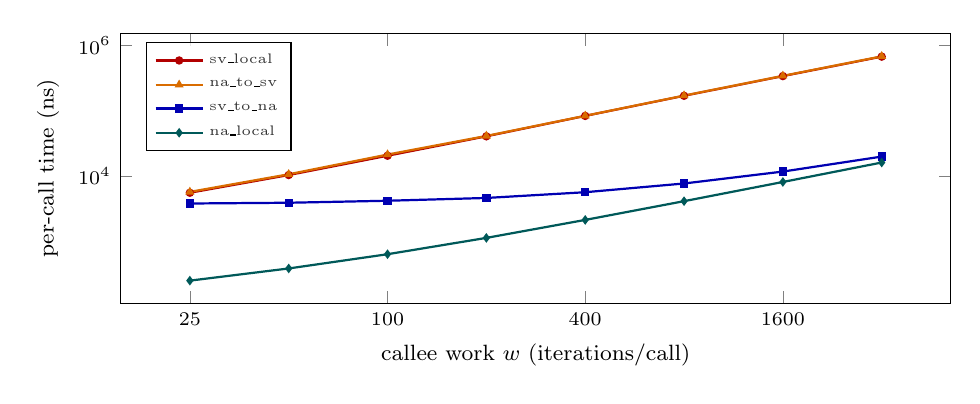
\begin{tikzpicture}
\begin{loglogaxis}[
  width=\columnwidth, height=5cm,
  log basis x=2,
  xlabel={callee work $w$ (iterations/call)},
  ylabel={per-call time (ns)},
  xtick={25,100,400,1600}, xticklabels={25,100,400,1600},
  legend pos=north west, legend style={font=\tiny, fill opacity=0.8},
  legend cell align=left,
  tick label style={font=\scriptsize}, label style={font=\footnotesize},
  every axis plot/.append style={thick, mark size=1.1pt},
]
\addplot[mark=*,red!70!black] coordinates {
  (25,5606)(50,10461)(100,20642)(200,40894)(400,83898)(800,170423)(1600,340780)(3200,676554)};
\addplot[mark=triangle*,orange!85!black] coordinates {
  (25,5781)(50,10752)(100,21526)(200,41460)(400,84280)(800,171498)(1600,343812)(3200,683614)};
\addplot[mark=square*,blue!70!black] coordinates {
  (25,3841)(50,3944)(100,4231)(200,4668)(400,5713)(800,7770)(1600,11820)(3200,20032)};
\addplot[mark=diamond*,teal!70!black] coordinates {
  (25,254)(50,390)(100,644)(200,1144)(400,2155)(800,4168)(1600,8194)(3200,16257)};
\legend{sv\_local,na\_to\_sv,sv\_to\_na,na\_local}
\end{loglogaxis}
\end{tikzpicture}
\caption{\code{iop\_symmetric}'s four placements. The two \code{sv}-executing
variants (\code{sv\_local}, \code{na\_to\_sv}) share the steep $\approx$$212$\,ns/it
slope; the two \code{na}-executing variants (\code{sv\_to\_na}, \code{na\_local})
share the shallow $\approx$$5$\,ns/it slope. \code{sv\_to\_na} sits a constant
$\approx$$3.7$\,\textmu s \emph{above} \code{na\_local}---that vertical offset is
the crossing intercept. Slope is placement; the offset is the boundary.}
\label{fig:placement}
\end{figure}

\subsection{Payload-cardinality scaling}
\label{sec:payload}

The family-1 sweep varies \emph{callee work} at fixed payload; the complementary
axis---\emph{payload size} at fixed work---is what turns a cross-runtime floor
into a per-element serialization curve. \code{xop\_feed\_payload} sweeps it: a
loopback \code{sv$\rightarrow$sv} RPC (\code{rpc}) and its in-process twin
(\code{direct}) each return a \code{list[$N$]} of \code{int} from the same
provider, with $N$ swept across sixteen sizes from $1$ to $100{,}000$ elements at a
fixed $20$ calls. Both sides run the identical \code{feed\_batch} LCG generator,
so at every $N$ the returned lists are byte-identical: the oracle passed at all
sixteen sizes (Table~\ref{tab:payload}), extending the differential-identity
witness across five orders of magnitude of payload and confirming the wire
round-trip preserves the list exactly.

Both paths fit $t(N)\approx t_0 + s\cdot N$ per call, but with opposite dominant
terms. The \code{direct} path is a near-perfect line of slope $s=342$\,ns/element
(95\% CI $339$--$343$, $R^2>0.9999$ over the whole range, run-to-run CV $0.1\%$):
building an $N$-element list in-process costs essentially just per-element
construction, with a negligible fixed floor ($\approx$$0.4$\,\textmu s intercept).
The \code{rpc} path is the mirror
image---a $\approx$$15$\,ms fixed per-call cost dominates at small $N$, and the
per-element serialization slope is buried beneath it until the payload grows
large. Over the full range the \code{rpc} fit is $s=890$\,ns/element (95\% CI
$848$--$983$) on a $\approx$$15$\,ms floor ($R^2=0.994$), measured directly
across the range rather than extrapolated from below break-even. That is
the result: \emph{crossing the RPC boundary costs $\approx$$2.6\times$ per element
what the in-process list costs} ($890$ vs.\ $342$\,ns/element)---the
JSON-encode/HTTP/decode marshalling tax laid bare as a slope, exactly the quantity
the family-1 method isolates, now measured on payload rather than work. The
consequence is visible in the ratio column of Table~\ref{tab:payload}: it
collapses from $\approx$$19{,}500\times$ at $N{=}1$ to $\approx$$3\times$ at
$N{=}100{,}000$---the inverse of the \code{iop\_cb} decay. There a fixed boundary was amortized by
growing \emph{work}; here a fixed RPC floor is amortized by growing \emph{payload},
while the direct twin it is measured against grows linearly.

Crucially, the crossing is now \emph{observed}, not inferred, and it reproduces:
the sweep was run three times end to end under the pinned clock, and the fit
coefficients are stable run to run---the \code{direct} slope at CV $0.1\%$, the
\code{rpc} serialization slope at CV $1.8\%$ ($871$--$911$\,ns/element), the
\code{rpc}/\code{direct} ratio at CV $1.8\%$. The one noisy term is the fixed-cost
floor (CV $7.2\%$, $14.6$--$17.0$\,ms), which the decomposition of
Table~\ref{tab:rpcfloor} attributes to application-server dispatch plus
\code{sv~import} client marshalling---a property of the hosted deployment path,
not the serialization boundary---and which does not touch the slope. Coefficients are also reported with a within-run
bootstrap CI (percentile pairs bootstrap over the sixteen sweep points, $B{=}10^4$).
The break-even payload at which the serialization term equals the fixed cost is
$N\approx17{,}000$ elements, and the sweep measures $N$ nearly six times beyond
it: at $N{=}100{,}000$ the slope term ($\approx$$89$\,ms) is $\approx$$5.9\times$
the $\approx$$15$\,ms fixed cost, so the crossing is firmly
\emph{slope-dominated}. The loopback RPC is a fixed-cost floor at small payloads
that hands off to a serialization curve at large ones, with the handoff directly
witnessed. The per-point crossing medians stay wide at
small $N$, where the fixed-cost floor's noise dominates: the \code{rpc} medians are
non-monotone for $N\le100$ and become strictly monotone from $N{=}250$ onward---%
exactly where the slope begins to emerge.

\begin{table}[t]
\caption{\code{xop\_feed\_payload}: per-call time returning a \code{list[$N$]}
over a loopback \code{sv$\rightarrow$sv} RPC vs.\ in-process, $N$ swept $1$ to
$100{,}000$ at $20$ calls; per-cell values are the median of three pinned-governor
sweeps at $n{=}20$ interleaved invocations per size (Section~\ref{sec:controls}).
Every row's \code{direct} and \code{rpc} canonical digests were byte-identical
($\checkmark$). \code{direct} fits $342$\,ns/element ($R^2{>}.9999$, run-to-run CV
$0.1\%$); \code{rpc} fits a $\approx$$15$\,ms fixed cost plus an $890$\,ns/element
serialization slope (95\% CI $848$--$983$, $R^2{=}.994$, run-to-run CV $1.8\%$),
the slope directly observed to overtake the fixed cost at $N\approx17{,}000$.
Per-run data are in \code{payload\_noturbo\_n20\_rep\{1,2,3\}.json}.}
\label{tab:payload}
\centering
\small
\begin{tabular}{@{}rrrrc@{}}
\toprule
$N$ & \code{direct} (\textmu s) & \code{rpc} (ms) & rpc/direct & dig. \\
\midrule
1      & $0.75$   & $14.6$ & $19{,}502\times$ & $\checkmark$ \\
10     & $3.98$   & $13.5$ & $3{,}398\times$  & $\checkmark$ \\
50     & $17.8$   & $15.0$ & $841\times$      & $\checkmark$ \\
100    & $34.4$   & $14.1$ & $410\times$      & $\checkmark$ \\
250    & $85.8$   & $14.9$ & $174\times$      & $\checkmark$ \\
500    & $171$    & $15.8$ & $93\times$       & $\checkmark$ \\
1000   & $347$    & $16.2$ & $47\times$       & $\checkmark$ \\
2000   & $689$    & $17.0$ & $25\times$       & $\checkmark$ \\
5000   & $1{,}711$ & $18.3$ & $11\times$      & $\checkmark$ \\
10000  & $3{,}410$ & $21.9$ & $6\times$       & $\checkmark$ \\
20000  & $6{,}795$ & $32.6$ & $5\times$       & $\checkmark$ \\
30000  & $10{,}171$ & $42.3$ & $4\times$      & $\checkmark$ \\
40000  & $13{,}584$ & $52.9$ & $4\times$      & $\checkmark$ \\
50000  & $17{,}026$ & $64.4$ & $4\times$      & $\checkmark$ \\
75000  & $25{,}539$ & $83.7$ & $3\times$      & $\checkmark$ \\
100000 & $34{,}293$ & $99.1$ & $3\times$     & $\checkmark$ \\
\bottomrule
\end{tabular}
\end{table}

\begin{figure}[t]
\centering
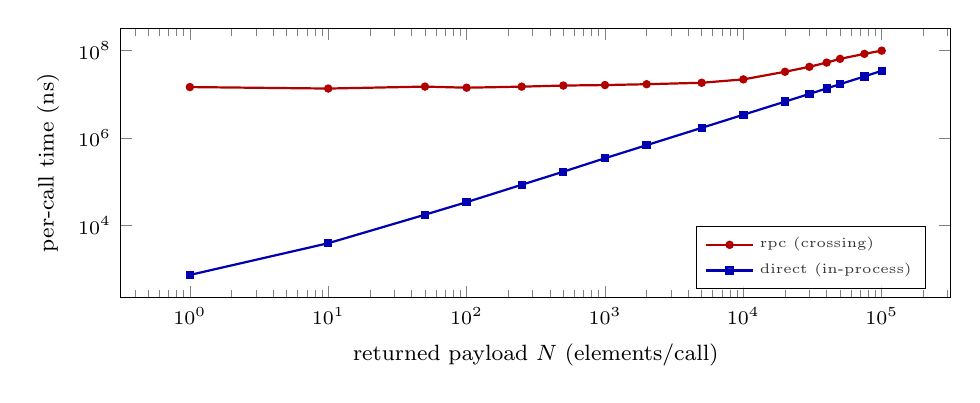
\begin{tikzpicture}
\begin{loglogaxis}[
  width=\columnwidth, height=5cm,
  log basis x=10,
  xlabel={returned payload $N$ (elements/call)},
  ylabel={per-call time (ns)},
  legend pos=south east, legend style={font=\tiny, fill opacity=0.8},
  legend cell align=left,
  tick label style={font=\scriptsize}, label style={font=\footnotesize},
  every axis plot/.append style={thick, mark size=1.1pt},
]
\addplot[mark=*,red!70!black] coordinates {
  (1,14606736)(10,13511981)(50,14968466)(100,14122879)(250,14925034)(500,15819482)(1000,16229288)(2000,16963593)(5000,18311699)(10000,21855446)(20000,32645548)(30000,42324280)(40000,52900132)(50000,64394525)(75000,83659745)(100000,99055558)};
\addplot[mark=square*,blue!70!black] coordinates {
  (1,749)(10,3977)(50,17795)(100,34448)(250,85831)(500,170755)(1000,346525)(2000,688588)(5000,1711470)(10000,3409932)(20000,6795209)(30000,10170737)(40000,13584290)(50000,17026283)(75000,25538996)(100000,34292691)};
\legend{rpc (crossing),direct (in-process)}
\end{loglogaxis}
\end{tikzpicture}
\caption{Payload-cardinality sweep, $N{=}1$ to $100{,}000$ (median of three pinned
sweeps). \code{direct} is a clean slope-$1$ line ($342$\,ns/element); \code{rpc}
is a flat $\approx$$15$\,ms floor that rises once the $890$\,ns/element
serialization term climbs above it, directly crossing break-even at
$N\approx17{,}000$. The two curves converge as $N$ grows---the crossing's fixed
cost amortizes over a larger payload while the in-process twin grows
linearly---and by $N{=}100{,}000$ the crossing is slope-dominated
($\approx$$5.9\times$ the fixed cost).}
\label{fig:payload}
\end{figure}

\section{Threats to Validity}
\label{sec:threats}

The differential-identity and structural-audit layers are the load-bearing
parts, and they are strong: byte-identical digests across every twin group and
matching manifest/wrapper facts are real correctness and compiler-regression
witnesses. The \emph{performance} layer is narrower than the kernel names
suggest, and we state its limits plainly.

\emph{Placement vs.\ boundary.} At a single size, \code{iop\_call} and
\code{iop\_symmetric} conflate \emph{which runtime runs the work} with crossing
cost. The size sweep (Section~\ref{sec:sweep}) separates the two---slope is
execution, intercept is crossing---but the separation is a linear extrapolation:
absolute intercepts are noisy (some slightly negative), so we quote only the
robust intercept \emph{gap} between twinned variants and the intercept of the
\code{sv\_to\_na} crossing, never a bare single-variant $t_0$.

\emph{FFI floors are not pure ABI.} \code{iop\_ffi\_scalar} includes two numeric
conversions per iteration; \code{iop\_ffi\_struct}'s $17$\,ns is an
\emph{average} across five struct shapes and must be split by shape before any
per-ABI-class claim.

\emph{Cross-runtime cells are floors, not workloads.} \code{xop\_feed} is a
\emph{sequential scalar} generated-client floor---no typed feed records and no
serialization-scaling measurement on that cell; it is not a HyperProtoBench-style
curve, and it measures a minimal custom \code{fetch} shim, not the shipped
\code{@jac/runtime}. The payload-scaling axis it lacks is supplied by the
separate \code{xop\_feed\_payload} sweep (Section~\ref{sec:payload}), which does
grow $N$ to $100{,}000$ elements over a loopback RPC; that cell in turn stays on a
\code{sv$\rightarrow$sv} loopback rather than a generated cross-language client,
so the two remain complementary floors rather than one production feed.
\code{xop\_wasm\_call} compares a Python-loop$\rightarrow$native-bridge against a
JavaScript-loop$\rightarrow$wasm-export---\emph{not} the same source built native
and wasm under equal host loops.

\emph{One machine; both axes now swept, payload fit with bootstrap intervals.} The family-1 mixed-JIT
cells are swept across eight callee-work sizes and fit to a fixed-cost intercept
plus an execution slope (Section~\ref{sec:sweep}); the complementary
\emph{payload-bytes} axis is measured by
\code{xop\_feed\_payload} across sixteen cardinalities to $100{,}000$ elements
(Section~\ref{sec:payload}), separating the loopback RPC's $\approx$$15$\,ms fixed
cost from its $890$\,ns/element serialization slope, reproducible across three
pinned sweeps (slope run-to-run CV $1.8\%$). The slope's within-run bootstrap CI
is $848$--$983$\,ns/element and the crossing is directly observed to cross
break-even at $N\approx17{,}000$ and reach $\approx$$5.9\times$ slope-dominance by
$N{=}100{,}000$. One caveat remains: the per-point crossing medians are wide at
small $N$, noise that lives in the fixed-cost floor, not the slope. Family-2
cross-runtime cells are now medians of three pinned runs at $n{=}20$ with
reported spread rather than a single warm-up, but the Node invocations still do
not guarantee stable V8 tiering and the RPC crossing-side IQRs are wide. Outside
the payload cell's fit CIs, results are one machine and report spread without
confidence intervals. None of these should be published as general Jac interop
overhead, realistic feeds, production microservices, or native-vs-wasm results.

We regard this candor as a feature. A benchmark suite for a language whose thesis
is measurable interop earns trust by naming exactly what each number licenses,
and by gating regressions on the facts it can defend (semantics and structure)
rather than the ones it cannot (absolute time on a shared runner).

\section{Design Implications}
\label{sec:implications}

The characterization is a means, not an end. Its purpose is to make the cost of
each boundary a quantity a compiler can \emph{act on}. Because a synechic
compiler owns both sides of every crossing, it already knows each call's
direction, static payload shape, and call-site frequency at compile time---the
exact inputs Table~\ref{tab:profiles} keys on. What the numbers here begin to
supply is the missing term: the per-crossing cost against which a placement or
marshalling decision pays off.

Three implications follow. The first two the sweep now quantifies; the third
remains a hypothesis. \emph{(i)~Placement is a slope; the crossing is an
intercept.} The sweep (Section~\ref{sec:sweep}) shows the two are literally
separable coefficients of one line: execution placement is a
$\approx$$42\times$ \emph{slope} difference ($5$ vs.\ $212$\,ns/iter) while the
crossing is a fixed \emph{intercept} ($\approx$$2.0$\,\textmu s for the
\code{iop\_cb} callback, $\approx$$3.7$\,\textmu s to enter \code{na}). A
compiler can therefore choose placement on callee slope alone once the intercept
is known small---and it can compute the exact break-even, which our fits make
concrete: entering \code{na} costs the $\approx$$3.7$\,\textmu s intercept and
saves $\approx$$207$\,ns/iter ($212$ minus $5$), so \emph{crossing into native
pays for itself above $\approx$$18$ iterations of callee work per call}. Below
that, stay in \code{sv}; above it, cross---a threshold computable at compile time
from the call's static work estimate. \emph{(ii)~The $\mu$s-vs-ns gap
sets a batching threshold.} A loopback RPC costs $\sim$$10^{7}$\,ns per call
while an in-process dispatch costs $\sim$$10^{4}$--$10^{5}$; the break-even call
count above which batching or computation-migration wins is the ratio Table~%
\ref{tab:xruntime} brackets ($\sim$$10^2$, from its batch-of-$20$ medians). Applying the intercept/slope method
to \emph{payload} rather than work makes the two terms concrete
(Section~\ref{sec:payload}): the loopback RPC resolves into a $\approx$$15$\,ms
fixed cost plus an $890$\,ns/element serialization slope---$2.6\times$ the
in-process list's $342$\,ns/element---so a compiler that knows a call's static
payload cardinality can compute both when the crossing amortizes (large $N$) and
what each additional element on the wire will cost. \emph{(iii)~ABI class is a codegen choice,
not a constant.} The
$2$\,ns scalar vs.\ $17$\,ns struct-by-value gap is exactly the register-vs-%
\code{byval} distinction a compiler resolves per call signature. The decision
tree these imply---direct FFI, copied FFI, batched FFI, RPC, or migrate the
computation into the target codespace---is the natural next system contribution;
this paper supplies its measurement substrate and leaves the selector itself as
future work.

\section{Related Work}
\label{sec:related}

The Computer Language Benchmarks Game~\cite{clbg} and PolyBench~\cite{polybench}
compare language \emph{implementations} on shared kernels; JacInteropBench instead
holds the language fixed and varies the \emph{boundary}, so its unit is one Jac
program crossing one marshalled seam, not two languages solving one problem.
gRPC's benchmark methodology~\cite{grpc} separates fixed per-call cost from
per-byte work---the intercept/slope decomposition we implement over callee work
for the family-1 cells (Section~\ref{sec:sweep}) and over payload cardinality for
\code{xop\_feed\_payload} (Section~\ref{sec:payload}), which resolves a loopback
RPC into a $\approx$$15$\,ms fixed cost and an $890$\,ns/element serialization
slope, observed to cross break-even at $N\approx17{,}000$. HyperProtoBench~\cite{hyperproto} characterizes serialization at scale;
our payload sweep is a minimal instance of that payload-growing axis, still on a
loopback \code{sv$\rightarrow$sv} seam rather than realistic proto messages. TechEmpower~\cite{techempower} defines realistic web-endpoint
workloads that a future \code{xop\_crud} would slice. The manually engineered interop these boundaries replace has its own
tooling---\code{ctypes} and CFFI, pybind11~\cite{pybind11} and
PyO3~\cite{pyo3} for Python$\leftrightarrow$native, FastAPI and generated
OpenAPI clients for \code{cl}$\rightarrow$\code{sv}. A differential comparison
against these---same computation, same data representation, Jac-generated
crossing vs.\ hand-written glue---is the axis that would turn our
\emph{characterization} into a \emph{verdict} on compiler-generated interop.
Section~\ref{sec:xtool} takes one step onto that axis, adding matched pybind11,
PyO3, and raw C-extension points to the \code{sqrt} kernel and explicitly
separating mechanism cost from CPython dispatch; the \emph{full} matrix (FastAPI
and generated OpenAPI clients for the RPC axis, more kernels, per-system warm-up
controls) remains the follow-on paper. We are careful there not to attribute host-interpreter dispatch
to the binding mechanism---the confound that a single matched number would
smuggle in. Within Jac, \code{ownbench}
covers the free single-runtime boundary and the memory-management dial; this suite
is its marshalled-boundary complement, sharing its output contract, oracle
discipline, and compiler-regression role. The GraalVM/Truffle line~\cite{graal} is the closest prior ``one runtime, many
languages'' interoperability work, but it measures a shared managed VM's
polyglot call layer; JacInteropBench instead measures a compiler that lowers
\emph{to distinct runtimes} (Python bytecode, JavaScript, native/wasm) and so
must characterize genuinely heterogeneous boundaries. Our \code{xop\_wasm\_call}
caveat is precisely the confound Jangda et al.~\cite{jangda} isolate at scale
(wasm vs.\ native under matched host loops), which is why we report ours as an
asymmetric floor rather than a codegen verdict. On statistics, we follow the
spirit of rigorous performance evaluation~\cite{georges,renaissance} by
reporting full spread per cell, run-to-run coefficients of variation across three
pinned-clock repetitions, and bootstrap confidence intervals for the payload-sweep
fit coefficients---while declining to manufacture intervals for the single-size
cells that a median of three $n{=}20$ runs does not support---and gating
regressions on semantics, not time. To our knowledge no
established suite targets ``Python $\leftrightarrow$ WebAssembly
$\leftrightarrow$ native in one language,'' because until synechic compilation
there was no single language spanning those runtimes to measure.

\section{Conclusion}
\label{sec:conclusion}

Taken together, the results say one thing about \emph{where} interop cost lives,
and one thing about \emph{how} to measure it. On magnitude: execution
\emph{placement} (a $\approx$$42\times$ slope) dwarfs the boundary crossing itself
(a fixed few $\mu$s), and for cross-runtime cells the \emph{deployment} path---the
application server and client stack---dwarfs the marshalling it wraps. The
actionable ordering is therefore placement first, deployment path second, boundary
mechanism last. On method: several of the suite's most striking-looking numbers
are, on inspection, deflations, and that is the contribution. The
``$5.4$\,\textmu s callback constant'' and the smooth $1.73\times$ decay were
CPU-frequency artifacts ($\approx$$2.0$\,\textmu s and noise once pinned); the
``$100\times$-class'' FFI win over pybind11-family bindings is $\approx$$10\times$
once interpreter dispatch is isolated from mechanism (a $25$--$54$\,ns boundary
band, only \code{ctypes} truly $100\times$-class); and the $374\times$/$241\times$
RPC floors are properties of Jac's hosted deployment path, not of an RPC boundary
in general. What survives every deflation is a small set of reproducible
\emph{ratios}---placement $42\times$, serialization $2.6\times$, the fixed-versus-%
slope decompositions---whose absolute nanoseconds are clock- and machine-specific
but whose shape is not. The differential-identity oracle, evaluated against $21$
seeded faults ($14/14$ result-corrupting crossings caught at CI sizes, three
escapes that delimit its scope), and frequency pinning as its timing-side
analogue, are what make those ratios trustworthy enough to quote.

Synechic compilation turns interop cost from an emergent property of hand-written
glue into a measurable property of one compiler. JacInteropBench is the
instrument for that measurement: ten measured kernels across two harness
families plus two named floors, each marshalled cell anchored to an exact
reference twin, a differential-identity oracle and structural audits gated in CI,
and provenance-stamped timing reported only within an explicitly bounded scope.
The work and payload sweeps above supply the coefficients; the oracle supplies
the trust. The suite's most durable output is not any single ratio but the
guarantee that every crossing stays byte-identical to its in-language reference on
every commit. Future work fits the
remaining shape---the payload method carried onto a typed cross-language
\code{xop\_feed} feed, plus concurrency and RPS on
\code{xop\_crud} and an arm64 C-ABI runner---each landing behind the same
twin-anchored, regression-gated contract.

\begin{thebibliography}{99}
\bibitem{jac} Jaseci Labs, ``The Jac Programming Language,''
\url{https://github.com/jaseci-labs/jaseci}, 2026.
\bibitem{clbg} I.\ Gouy, ``The Computer Language Benchmarks Game,''
\url{https://benchmarksgame-team.pages.debian.net/benchmarksgame/}.
\bibitem{polybench} L.-N.\ Pouchet, ``PolyBench/C: The Polyhedral Benchmark
Suite,'' \url{https://web.cse.ohio-state.edu/~pouchet.2/software/polybench/}.
\bibitem{grpc} gRPC Authors, ``gRPC Performance Benchmarking,''
\url{https://grpc.io/docs/guides/benchmarking/}.
\bibitem{hyperproto} A.\ Kolesnikov et al., ``HyperProtoBench: A Realistic
Protocol Buffer Serialization Benchmark,'' Google, 2020.
\bibitem{techempower} TechEmpower, ``Web Framework Benchmarks,''
\url{https://www.techempower.com/benchmarks/}.
\bibitem{pybind11} W.\ Jakob, J.\ Rhinelander, and D.\ Moldovan, ``pybind11---%
Seamless operability between C++11 and Python,''
\url{https://github.com/pybind/pybind11}, 2017.
\bibitem{pyo3} PyO3 Project, ``PyO3: Rust bindings for Python,''
\url{https://github.com/PyO3/pyo3}.
\bibitem{jangda} A.\ Jangda, B.\ Powers, E.\ D.\ Berger, and A.\ Guha, ``Not So
Fast: Analyzing the Performance of WebAssembly vs.\ Native Code,'' in
\emph{USENIX ATC}, 2019.
\bibitem{graal} M.\ Grimmer, C.\ Seaton, R.\ Schatz, T.\ W\"urthinger, and
H.\ M\"ossenb\"ock, ``High-performance Cross-language Interoperability in a
Multi-language Runtime,'' in \emph{DLS}, 2015.
\bibitem{georges} A.\ Georges, D.\ Buytaert, and L.\ Eeckhout,
``Statistically Rigorous Java Performance Evaluation,'' in \emph{OOPSLA}, 2007.
\bibitem{renaissance} A.\ Prokopec et al., ``Renaissance: Benchmarking Suite
for Parallel Applications on the JVM,'' in \emph{PLDI}, 2019.
\bibitem{mytkowicz} T.\ Mytkowicz, A.\ Diwan, M.\ Hauswirth, and
P.\ F.\ Sweeney, ``Producing Wrong Data Without Doing Anything Obviously
Wrong!'' in \emph{ASPLOS}, 2009.
\end{thebibliography}

\end{document}
